\documentclass[journal,10pt,a4paper]{IEEEtran}
\usepackage{fontspec}
\setmainfont{Times New Roman}
\setsansfont{Arial}
\setmonofont{Consolas}[Scale=0.85]
\usepackage{xeCJK}
\setCJKmainfont{SimSun}[AutoFakeBold=2]
\setCJKsansfont{SimHei}
\setCJKmonofont{SimSun}
\usepackage{amsmath,amssymb}
\usepackage{graphicx,booktabs,array,tabularx}
\usepackage{float,stfloats,placeins,balance}
\usepackage{url}
\usepackage[hidelinks]{hyperref}
\newcolumntype{L}{>{\raggedright\arraybackslash}X}
\newcolumntype{C}{>{\centering\arraybackslash}X}
\providecommand{\tightlist}{\setlength{\itemsep}{0pt}\setlength{\parskip}{0pt}}
\newcommand{\pandocbounded}[1]{#1}
\renewcommand{\figurename}{图}
\renewcommand{\tablename}{表}
\renewcommand{\refname}{参考文献}
\emergencystretch=1em
\linespread{0.98}
\setlength{\textfloatsep}{10pt plus 2pt minus 2pt}
\setlength{\dbltextfloatsep}{10pt plus 2pt minus 2pt}
\setlength{\floatsep}{8pt plus 2pt minus 2pt}
\setlength{\dblfloatsep}{8pt plus 2pt minus 2pt}
\setlength{\intextsep}{8pt plus 2pt minus 2pt}
\setcounter{topnumber}{3}
\setcounter{dbltopnumber}{3}
\renewcommand{\topfraction}{.90}
\renewcommand{\dbltopfraction}{.90}
\renewcommand{\textfraction}{.08}
\renewcommand{\floatpagefraction}{.80}
\raggedbottom
\begin{document}

\title{补充材料：受控干预启发的极化与区域证据学习用于跨场景SAR船舶分类}\author{Mo Yu, Xiangguang Leng, \IEEEmembership{Member,~IEEE}, Qihao Huang, Jilong Li, and Kefeng Ji, \IEEEmembership{Member,~IEEE}\thanks{This work was supported in part by the National Natural Science Foundation of China under Grant 62471475, in part by Hunan Provincial Natural Science Foundation of China under Grant 2024JJ4045, and in part by the Science and Technology Innovation Program of Hunan Province under Grant 2024RC3124.}\thanks{M. Yu, X. Leng, Q. Huang, J. Li, and K. Ji are with the College of Electronic Science and Technology, National University of Defense Technology, Changsha 410073, China. Corresponding author: Xiangguang Leng (e-mail: luckight@163.com).}}\maketitle

\section{补充材料的范围}\label{ux8865ux5145ux6750ux6599ux7684ux8303ux56f4}

本文件独立于论文正文，提供同船诊断、受控干预实现、模块计算细节、源端初始化训练、配套组件分析及部署计算。正文主结果采用共享骨干与证据模块联合微调后的完整模型；下文按实验实际配置区分三类证据：

\begin{itemize}
\tightlist
\item
  全骨干微调：与正文当前主模型对应，查询和参考由当前共享编码器计算。
\item
  受限骨干训练与初始化：仅更新指定骨干层及证据模块，用于源端初始化与共同起点组件比较。
\item
  固定上游或固定权重替换：用于检验特定读出、参考消息或计算路径，不替代最终模型的配套重训。
\end{itemize}

本文件的图、表、公式独立编号。未完成实验的占位表保留在正文；本文件只列已有结果。历史配置的收益用于解释相应机制，不移作全骨干微调版的组件增量。

\section{数据与输入因素}\label{ux6570ux636eux4e0eux8f93ux5165ux56e0ux7d20}

\subsection{成像与预处理因素}\label{ux6210ux50cfux4e0eux9884ux5904ux7406ux56e0ux7d20}

\begin{table}[H]
\centering\footnotesize
\setcounter{table}{0}
\caption{影响Sentinel-1船舶表征的主要因素。}
\label{tab:1}
\setlength{\tabcolsep}{3pt}\renewcommand{\arraystretch}{1.2}
\begin{tabularx}{\linewidth}{LL}
\toprule
因素 & 对输入表征的影响 \\
\midrule
成像几何：入射角、相对方位 & 改变同一船舶的散射强度与空间分布 \\
船舶结构：船体、甲板、上层建筑 & 形成目标内部的局部散射差异 \\
极化与散射：VV/VH & 同一目标在两极化中的响应不同 \\
海洋环境：风浪、海况 & 改变海杂波与船海对比度 \\
船舶运动：航速、航向 & 可能产生方位向偏移或散焦，并影响尾迹形态 \\
数据集预处理：辐射定标、灰度拉伸、重采样与裁片 & 改变数值分布、船海对比度、局部纹理及目标／邻域覆盖，影响可用分类证据 \\
\bottomrule
\end{tabularx}
\end{table}

\subsection{港口与类别组成}\label{ux6e2fux53e3ux4e0eux7c7bux522bux7ec4ux6210}

自建数据覆盖24港、38,091条观测；下表的``诊断观测''指同船和输入分析使用的4,744条子集，不是最终分类测试集。最终测试集为3,075条观测。两种集合承担不同评价任务。

\begin{table}[H]
\centering\footnotesize
\setcounter{table}{1}
\caption{自建24港逐港组成及诊断覆盖。}
\label{tab:2}
\setlength{\tabcolsep}{3pt}\renewcommand{\arraystretch}{1.2}
\begin{tabularx}{\linewidth}{LCCC}
\toprule
港口 & 总库观测 & 实际类别数 & 诊断观测 \\
\midrule
Antwerp-Bruges & 886 & 3 & 0 \\
Busan & 871 & 3 & 48 \\
Callao & 476 & 8 & 14 \\
Fujairah & 1,158 & 3 & 178 \\
Hamburg & 1,619 & 3 & 0 \\
Houston & 804 & 8 & 9 \\
Jebel Ali & 4,602 & 8 & 1,046 \\
Los Angeles & 583 & 8 & 158 \\
Melbourne & 64 & 3 & 0 \\
Mombasa & 149 & 7 & 12 \\
New York & 470 & 8 & 0 \\
Newcastle & 299 & 7 & 25 \\
Ningbo-Zhoushan & 5,756 & 3 & 292 \\
Port Hedland & 859 & 6 & 53 \\
Port Klang & 3,425 & 8 & 1,238 \\
Port Said & 1,895 & 8 & 150 \\
Qingdao & 1,981 & 3 & 0 \\
Richards Bay & 744 & 8 & 241 \\
Rotterdam & 573 & 3 & 36 \\
Santos & 1,658 & 8 & 325 \\
Shanghai & 2,390 & 3 & 0 \\
Singapore & 5,259 & 8 & 821 \\
Sydney Botany & 304 & 8 & 10 \\
Tanger Med & 1,266 & 8 & 88 \\
合计 & 38,091 & 合计8类 & 4,744 \\
\bottomrule
\end{tabularx}
\end{table}

表3给出八类组成。诊断队列包含4,744条观测、2,973艘船和18港；同船最大日期跨度配对子集包含910艘船、1,820条观测，覆盖13港和7类。受控干预队列按本文件受控干预部分的条件另行组织。

\begin{table}[H]
\centering\footnotesize
\setcounter{table}{2}
\caption{自建数据集类别分布。}
\label{tab:3}
\setlength{\tabcolsep}{3pt}\renewcommand{\arraystretch}{1.2}
\begin{tabularx}{\linewidth}{LLL}
\toprule
船型 & 总库观测 & 诊断观测 \\
\midrule
散货船 & 11,128 & 1,290 \\
渔船 & 8,599 & 145 \\
普通货船 & 5,929 & 439 \\
化学品／成品油轮 & 5,827 & 1,480 \\
集装箱船 & 2,208 & 519 \\
原油轮 & 1,757 & 405 \\
拖轮／拖带船 & 1,478 & 202 \\
海工补给船 & 1,165 & 264 \\
合计 & 38,091 & 4,744 \\
\bottomrule
\end{tabularx}
\end{table}

\subsection{划分与源参考}\label{ux5212ux5206ux4e0eux6e90ux53c2ux8003}

根据产品元数据恢复平台与绝对轨道，合并同次过境的相邻产品切片，再划分训练集、验证集和测试集。三个集合之间隔离船舶身份及过境组，测试查询不使用目标标签。该协议以未见船舶和未见过境组织跨场景测试，地理水域随实际产品覆盖变化，不要求训练与测试来自完全不同的港口。自建24港的场景描述同时保留港口归属，以分析同港和异港条件下的观测差异。表4给出OSS2类别组成。

\begin{table*}[!t]
\centering\footnotesize
\setcounter{table}{3}
\caption{OSS2四分类划分。括号内为独立船数。}
\label{tab:4}
\setlength{\tabcolsep}{3pt}\renewcommand{\arraystretch}{1.2}
\begin{tabularx}{\linewidth}{LCCCCC}
\toprule
集合 & 散货船 & 普通货船 & 化学品/成品油轮 & 集装箱船 & 总观测/船数/过境 \\
\midrule
训练集 & 221（216） & 73（71） & 141（137） & 284（259） & 719 / 683 / 13 \\
验证集 & 87（84） & 23（22） & 29（29） & 89（88） & 228 / 223 / 4 \\
测试集 & 132（128） & 26（26） & 83（81） & 137（134） & 378 / 369 / 5 \\
\bottomrule
\end{tabularx}
\end{table*}

OSS2训练集进一步分为478条表征训练观测和241条干预适配观测。固定32个源参考，每类8个，均来自表征训练子集；测试集覆盖五个过境。

自建24港完整训练采用20,653条合法训练记录，其中19,981条用于表征训练、672条用于干预适配；验证集含160条观测、158艘船和3个过境，测试集含3,075条观测、1,950艘船和85个完整过境组。完整过境组由卫星平台、绝对轨道号及数据获取批次（datatake）共同确定；测试集对应81个平台---绝对轨道组合，其中4个组合各包含两个datatake。训练集覆盖24港，测试集覆盖18港，沿用既有身份与过境隔离划分。源参考共16艘，每类2艘。类别反馈和区域读出阶段各遍历训练数据两轮，其余阶段沿用相应训练配方。

\section{同船诊断与受控干预}\label{ux540cux8239ux8bcaux65adux4e0eux53d7ux63a7ux5e72ux9884}

\subsection{从自然不稳定到可检验问题}\label{ux4eceux81eaux7136ux4e0dux7a33ux5b9aux5230ux53efux68c0ux9a8cux95eeux9898}

同船诊断使用自建24港语料中的4744次观测、2973个船舶身份、18港及八个输出类别。对每艘具有重复观测的船选择日期跨度最大的一对，得到910艘船的1820次观测，覆盖七类。表5给出三种代表性船型的三种子平均状态比例。

\begin{table*}[!t]
\centering\footnotesize
\setcounter{table}{4}
\caption{同船重复观测的分类状态，三种子平均。}
\label{tab:5}
\setlength{\tabcolsep}{3pt}\renewcommand{\arraystretch}{1.2}
\begin{tabularx}{\linewidth}{LCCCC}
\toprule
船型 & 船对数 & 两次均正确（\%） & 一次正确一次错误（\%） & 两次均错误（\%） \\
\midrule
集装箱船 & 126 & 35.98 & 34.92 & 29.10 \\
原油轮 & 100 & 27.67 & 54.67 & 17.67 \\
普通货船 & 62 & 4.84 & 27.42 & 67.74 \\
\bottomrule
\end{tabularx}
\end{table*}

原油轮较多表现为观测相关的不稳定，普通货船则更多持续混淆。跨港与同港的粗比较还受到类别组成影响：未经类别等权，跨港``两次均错误''比例为38.80\%，低于同港43.92\%；按七类等权后分别为50.94\%和46.06\%，方向反转。因此，任务需同时关注观测条件与类别组成，不能把跨港分组差异直接解释成港口的独立效应。

在相同源划分和配套训练的Ridge读出下，整图输入与卷积前框内掩膜输入的OA/BA分别为35.139\%/38.795\%和32.610\%/37.231\%；原油轮召回分别为53.580\%和42.222\%。整图输入在4744条观测中纠正690条、误判新增570条，净增加120条正确判断。这表明外围可见响应包含可利用的补充信息，也具有误导风险，需要区分其对具体类别竞争的作用。

\subsection{干预定义与类别竞争}\label{ux5e72ux9884ux5b9aux4e49ux4e0eux7c7bux522bux7adeux4e89}

记双极化输入为 \(x=(x^{VV},x^{VH})\)，固定诊断器为 \(T\)，真实类别为 \(y\)。以原图最强错误类作为固定竞争类别 \(c^\star=\arg\max_{c\ne y}T_c(x)\)，定义分差及操作效应：

\[\begin{aligned}
m_{y,c^\star}(x)&=T_y(x)-T_{c^\star}(x),\\
\Delta m_a&=m_{y,c^\star}(x_a^I)-m_{y,c^\star}(x).
\end{aligned}\tag{1}\]

其中 \(a=(p,r,b)\) 指定极化 \(p\)、区域 \(r\) 和尺度 \(b\)。图像尺度分量取

\[D_f(I)=I-G_1(I),\qquad D_m(I)=G_1(I)-G_2(I).\tag{2}\]

\(G_\sigma\) 为标准差为 \(\sigma\) 个原生像素的高斯平滑。限定区域内通过平滑边缘掩膜削弱分量，保持另一极化、检测框、参考库和模型参数不变。结构操作使用共同 \(L_2\) 剂量，并设置具有相同区域净灰度变化的均值控制，以区分局部结构变化和平均亮度变化的作用。

式（1）可分解为 \(\Delta T_y-\Delta T_{c^\star}\)。因此，正确类分数下降并不必然意味着决策退化：如果错误竞争类下降更多，分差仍可改善。为排除竞争类切换造成的虚假改善，选样时进一步检查各自最强错误类定义的分差 \(m_{\max}(x)=T_y(x)-\max_{c\ne y}T_c(x)\)。

\subsection{极化与区域决定操作效应}\label{ux6781ux5316ux4e0eux533aux57dfux51b3ux5b9aux64cdux4f5cux6548ux5e94}

在自建24港语料的104艘船、209次观测、31个过境和6港干预队列中，VH框内细尺度削弱平均损害正确类别优势，VH侧向中尺度削弱平均改善优势，同一侧向中尺度操作在VV中则为负。表6以诊断器分差报告效应及船级95\%区间。

\begin{table}[H]
\centering\footnotesize
\setcounter{table}{5}
\caption{极化与区域干预的船均分差变化。}
\label{tab:6}
\setlength{\tabcolsep}{3pt}\renewcommand{\arraystretch}{1.2}
\begin{tabularx}{\linewidth}{LCCC}
\toprule
操作 & 平均 \(\Delta m\) & 船级95\%区间 & 相对同均值控制的剩余效应 \\
\midrule
VH框内细尺度削弱 & −0.003910 & {[}−0.005232, −0.002528{]} & −0.002997 \\
VH侧向中尺度削弱 & +0.002023 & {[}+0.000882, +0.003169{]} & +0.001417 \\
VV侧向中尺度削弱 & −0.001454 & {[}−0.002477, −0.000476{]} & −0.001147 \\
\bottomrule
\end{tabularx}
\end{table}

类别进一步调节操作效应：VH侧向中尺度削弱在9艘集装箱船上的平均分差变化为+0.008422，在7艘散货船上为−0.008180。相反的作用方向支持保留极化和区域身份，并依据类别响应学习取证方式。

\subsection{类别竞争的案例分析}\label{ux7c7bux522bux7adeux4e89ux7684ux6848ux4f8bux5206ux6790}

图1的散货船10488展示了类别竞争的变化。仅削弱VH框内细尺度后，散货分数增加0.11492，错误原油轮分数下降0.16278，分差提高0.27769；均值控制仍误判。对照案例化学品船26628则同时降低正确类并抬高海工竞争类，产生误伤。局部证据的效用因此需落实到正确类与竞争类的相对变化。

\begin{figure}[!htb]
\centering
\setcounter{figure}{0}
\includegraphics[width=\linewidth,height=.30\textheight,keepaspectratio]{figures/author_20261110/fig2_author.pdf}
\caption{散货船10488的受控干预与实际参考。上两行依次展示VV和VH，各列为原图、像素变化图、干预后图像及匹配均值控制；下方为实际同类与混淆类参考。VV保持不变，VH框内细尺度削弱改变类别竞争，均值控制仍误判。结果来自固定诊断模型。}
\label{fig:1}
\end{figure}

\section{模块计算细节}\label{ux6a21ux5757ux8ba1ux7b97ux7ec6ux8282}

\subsection{类别响应反馈模块（CRFB）}\label{ux7c7bux522bux54cdux5e94ux53cdux9988ux6a21ux5757crfb}

局部高响应可能同时支持多个易混淆类别，仅依据响应强弱进行重标定，难以描述它对类别竞争的不同作用。CRFB以当前类相对其他类的响应为条件，计算其与局部内容变化的关联，并将这种关联反馈至中间特征；均值支路同时保留整体上下文。

设某一极化的输入为 \(X_1(u)\in\mathbb R^{128}\)，\(u\)表示空间位置，有效面积占比为 \(o(u)\)，归一化权重为 \(\omega(u)=o(u)/\sum_v o(v)\)。屏蔽无效位置后，以两个 \(1\times1\) 卷积得到32维值特征 \(V_1(u)\) 和 \(K\) 维候选类别响应 \(A(u)\)。记 \(\bar V_1=\sum_u\omega(u)V_1(u)\)，相对类别响应及其标准化量为

\[\begin{aligned}
d_k(u)&=A_k(u)-\frac{1}{K-1}\sum_{j\ne k}A_j(u),\\
\bar d_k&=\sum_u\omega(u)d_k(u),\\
s_k(u)&=\frac{d_k(u)-\bar d_k}
{\sqrt{\sum_v\omega(v)(d_k(v)-\bar d_k)^2+0.01}}.
\end{aligned}\tag{3}\]

以相对响应和局部值的共同变化形成类别相关摘要：

\[\begin{aligned}
C_k&=\sum_u\omega(u)\,[V_1(u)-\bar V_1]s_k(u),\\
R_1(u)&=\frac1K\sum_k\tanh(s_k(u))\tanh(L_k(C_k)).
\end{aligned}\tag{4}\]

\(C_k\)描述低维内容与标准化类别响应之间的交叉统计，\(L_k\)为含偏置的仿射映射。令均值变换 \(U_0=W_0\tanh(L_0(\bar V_1))\)，与关系支路共同生成有界门控并反馈至原特征：

\[\begin{gathered}
G_{\mathrm{CRFB}}(u)=o(u)\tanh\{U_0+W_1R_1(u)\},\\
X'_1(u)=X_1(u)+0.3X_1(u)\odot G_{\mathrm{CRFB}}(u).
\end{gathered}\tag{5}\]

输出映射零初始化，使训练从原特征路径开始。类别辅助读出利用源标签约束候选响应。\(X'_1\)经过该block的conv3、归一化与残差相加形成layer2输出 \(F_2\)；类别响应保留给后续区域读出使用。

\begin{figure*}[!tb]
\centering
\setcounter{figure}{1}
\includegraphics[width=\linewidth,height=.40\textheight,keepaspectratio]{figures/author_20261110/fig4_author.pdf}
\caption{CRFB。当前类相对其他类均值的响应经标准化，与内容形成交叉统计 \(C_k\)，再与内容均值分别变换并生成局部门控。输出投影恢复128通道，反馈增益为0.3，有效面积占比屏蔽补零位置。}
\label{fig:2}
\end{figure*}

式（4）中的交叉统计同时包含内容偏离和类别响应偏离，反馈因而不只依赖某个位置的激活大小。相比CAM的类别激活定位{[}14{]}与GSoP的特征统计重标定{[}17{]}，这里将候选类别相对响应与中心化局部内容关联起来，形成位置相关的中间层更新。CRFB输出的类别响应还继续用于RGRP，在特征反馈与区域取证之间共享判别依据。

\subsection{响应引导区域池化（RGRP）}\label{ux54cdux5e94ux5f15ux5bfcux533aux57dfux6c60ux5316rgrp}

统一的全局汇总会压缩船体与不同方向外围的空间差别，而预先划定区域也不能保证区域内各位置具有相同的判别价值。RGRP结合目标几何与CRFB类别响应，分别处理``从哪个区域读取''及``区域内如何加权''两个问题。该模块包含骨干内部的区域池化回写，以及面向分类的多层区域读出。

\subsubsection{区域身份与内部回写}\label{ux533aux57dfux8eabux4efdux4e0eux5185ux90e8ux56deux5199}

以OBB长轴建立目标相对坐标，构造框内、轴端与侧向三个区域。框内为长宽 \(L,W\) 的软矩形；轴端为长轴扩展至 \(1.5L\) 的矩形减去框内；侧向为宽度扩展至 \(2W\) 的矩形减去框内。区域与有效输入范围相交，以特征网格实际面积占比表示 \(m_r(u)\)。两轴端对称处理，无需船首、船尾标注。

对于特征 \(F\)，区域均值为

\[\pi_r(u)=\frac{m_r(u)}{\sum_v m_r(v)},\qquad \operatorname{Pool}_r(F)=\sum_u\pi_r(u)F(u).\tag{6}\]

令 \(t_r=\operatorname{Pool}_r(X_3)\)。空区域返回零并屏蔽更新。layer3{[}5{]}中的内部RGRP以区域专属两层映射 \(\phi_r\) 变换摘要，只回写至相应区域：

\[\begin{gathered}
X'_3(u)=X_3(u)+\sum_r\widetilde m_r(u)\phi_r(t_r),\\
\widetilde m_r(u)=m_r(u)/\max\{1,\sum_jm_j(u)\}.
\end{gathered}\tag{7}\]

其中 \(X_3\) 为conv1激活后的256通道特征。区域专属变换保留框内、轴端与侧向的身份，不将三者合成同一个上下文再广播到全图。回写保持空间尺寸，使随后 \(3\times3\) 卷积同时读取局部内容与对应区域的摘要。另两处区域读出仅汇总特征，用于最终分类。

\subsubsection{由CRFB响应指导浅层取证}\label{ux7531crfbux54cdux5e94ux6307ux5bfcux6d45ux5c42ux53d6ux8bc1}

CRFB读取layer2{[}3{]}中的128通道特征，其响应与该block末端512通道特征 \(F_2\) 位于同一 \(20\times20\) 网格。在有效范围内标准化相对类别响应，得到有界评分 \(q_k(u)=2\tanh(s_k(u))\)。在每个区域内分别归一化：

\[\begin{aligned}
\alpha_{r,k}(u)&=\frac{m_r(u)\exp q_k(u)}{\sum_v m_r(v)\exp q_k(v)},\\
t_{r,k}&=\sum_u\alpha_{r,k}(u)V_2(u).
\end{aligned}\tag{8}\]

其中 \(V_2=W_V^{(2)}\operatorname{LN}(F_2)\) 为512维到32维的值投影。同时保留均匀摘要 \(t_{r,0}=\sum_u\pi_r(u)V_2(u)\)；四类时五个摘要拼接为160维。记 \(t_r^{\mathrm{cat}}=[t_{r,0};\ldots;t_{r,K}]\)，\(\sigma_{p,r}=\operatorname{stopgrad}\{\operatorname{RMS}(\operatorname{Pool}_r(F_{2,p}))\}\)，补充量为

\[\delta^{(2)}_{p,r}=0.1\sigma_{p,r}\tanh(W_p^{\mathrm{read}}t_r^{\mathrm{cat}}).\tag{9}\]

\(W_p^{\mathrm{read}}\)将 \(32(K+1)\) 维映射回512维，四分类时输入为160维，八分类时为288维；该映射零初始化，同一极化的三区域共享。所有候选类别同时参与，既不输入查询真值，也不按当前预测的单一类别硬路由。输出仍位于原有区域槽位，保留均值信息，并用有界残差限制新增路径的幅度。式（8）回答``在这一几何区域内哪些位置更有助于类别区分''，式（6）回答``该区域总体包含什么''。

\begin{figure}[!htb]
\centering
\setcounter{figure}{2}
\includegraphics[width=\linewidth,height=.30\textheight,keepaspectratio]{figures/author_20261110/fig5_author.pdf}
\caption{CRFB引导的RGRP浅层读出，以四分类为例。类别响应 \(A(u)\) 与内容投影 \(V_2(u)\) 在区域内联合取证；均值及类别加权摘要拼接，经160到512维投影和有界变换形成补充量。区域归一化权重为 \(\pi_r\)，补充增益为0.1，尺度参照采用停止梯度的RMS。}
\label{fig:3}
\end{figure}

区域权重依据特征中心的覆盖面积计算；由于卷积感受野交叠，区域描述保留的是计算位置与目标几何的关系。

\subsection{参考类别证据回写（RCEW）}\label{ux53c2ux8003ux7c7bux522bux8bc1ux636eux56deux5199rcew}

CRFB和RGRP主要组织当前图像内部的证据；当查询中某些局部响应同时接近多个船型时，还需要比较它与不同类别参考之间的关系。RCEW利用固定源参考库构造这种比较，将``局部内容更接近哪类参考、相对其他类优势多大''转化为类别证据场，再反馈至骨干。参考信息因此参与后续特征计算，而不只提供末端相似度分数。

\subsubsection{比较描述与值描述分离}\label{ux6bd4ux8f83ux63cfux8ff0ux4e0eux503cux63cfux8ff0ux5206ux79bb}

RCEW使用源参考库补充单图判别。首先对当前共享骨干的layer1和layer2特征分别读出区域局部描述，通道数为256和512。每极化各自投影至32维并拼接，再分别生成32维比较键 \(k\) 与值 \(v\)。键经归一化用于比较，值用于构造判别消息。局部槽位保留框内8、侧向8、轴端4的组织，空槽和不可用极化不参与参考比较。

正式模型联合微调时，查询与参考使用当前骨干重新计算特征。固定上游读出实验使用共同锚点表示，适用于该项机制比较。

对某区域的合法源参考，按参考标签形成类均值 \(\mu_c\) 和其他类均值 \(\mu_{\neg c}\)，记 \(a_c=[\mu_c;\mu_{\neg c};\mu_c-\mu_{\neg c}]\)，由共享小网络生成有界正通道度量：

\[\begin{gathered}
w_c=1+0.5\tanh\psi(a_c),\\
S_{sij}=\cos(\sqrt{w_{y_s}}\odot k_i^q,\sqrt{w_{y_s}}\odot k_{sj}^{\mathrm{ref}}).
\end{gathered}\tag{10}\]

这里 \(i,j\) 分别是查询与参考的局部槽位，\(s\)是参考船，\(y_s\)是已知源标签；为简洁省略极化和区域索引。通道分支以32维类均值、其他类均值及其差拼接为96维，经96→16→32的小网络生成 \(w_c\in(0.5,1.5)^{32}\)。它既用于键的加权余弦比较，也用于后续值距离，并非独立的分类头。

空间分支先计算查询槽位对类别 \(c\) 的最佳相似度 \(B_{ic}=\max_{s:y_s=c,j}S_{sij}\)，只在合法参考和非空槽位上取最大值。再以 \(b_{ic}=B_{ic}-\operatorname{mean}_{c'\ne c}B_{ic'}\) 表示相对其他可用类的优势，形成比较logit \(L_{sij}=S_{sij}+b_{i,y_s}\)。只有一个可用类别时令 \(b_{ic}=0\)。带未匹配槽的Sinkhorn归一化产生有效传输 \(T_s\)，非法位置在归一化前屏蔽。通道与空间分支因此是耦合的比较步骤，而不是两个结果直接相加的独立分支。

\begin{figure*}[!tb]
\centering
\setcounter{figure}{3}
\includegraphics[width=\linewidth,height=.40\textheight,keepaspectratio]{figures/author_20261110/fig6_author.pdf}
\caption{RCEW比较、类别聚合与证据回写。通道度量参与空间相似度，本类最佳相似度相对其他类最佳相似度均值的优势调节传输。比较路径保留原传输，值路径采用边际外积聚合。行边际 \(\rho_{si}\) 对应查询槽位，列边际 \(\kappa_{sj}\) 对应参考槽位，外积除以有效总质量 \(M_s\)。64维描述包含逐层投影，值距离取负并经温度缩放和类别中心化形成证据，再经空间分配和1×1映射残差回写。}
\label{fig:4}
\end{figure*}

\subsubsection{类别条件的参考聚合}\label{ux7c7bux522bux6761ux4ef6ux7684ux53c2ux8003ux805aux5408}

记 \(T_s\) 的有效行、列边际为 \(\rho_{si}=\sum_jT_{sij}\)、\(\kappa_{sj}=\sum_iT_{sij}\)，有效总质量为 \(M_s=\sum_i\rho_{si}\)。选用的聚合版在值传递阶段使用

\[T^{\mathrm{agg}}_{sij}=\frac{\rho_{si}\kappa_{sj}}{M_s},\qquad \bar v_s=\frac{\sum_j\kappa_{sj}v^{\mathrm{ref}}_{sj}}{M_s}.\tag{11}\]

上述等式适用于分母非零的位置，其余位置屏蔽。\(\bar v_s\)实际是按列边际汇总的区域参考值，不再保留查询槽位到参考槽位的一一精细搬运。参考权重仍依赖原传输与相似度：先计算 \(g_{si}=\sum_jT_{sij}S_{sij}/\rho_{si}\)，再在合法参考间令 \(\beta_{si}=\operatorname{softmax}_s(g_{si}/0.1)\)。类参考表示为

\[P_{ic}=\frac{\sum_{s:y_s=c}\beta_{si}\bar v_s}
{\sum_{s:y_s=c}\beta_{si}}. \tag{12}\]

边际聚合保留查询相关的参考选择及类内组织，将局部值对应压缩为区域参考摘要。这样，比较路径负责确定值得参考的响应及参考样本，值路径则以类别为单位汇总可传递的内容；二者通过传输边际和参考权重相联系。

\subsubsection{类别证据场及空间回写}\label{ux7c7bux522bux8bc1ux636eux573aux53caux7a7aux95f4ux56deux5199}

查询值与各类参考表示的距离形成候选类别证据，取 \(e_{ic}=-D_{ic}/0.1\)，并在可用类别中中心化：

\[\begin{gathered}
D_{ic}=\sum_d w_{c,d}(v^q_{i,d}-P_{ic,d})^2,\\
\widetilde e_{ic}=e_{ic}-\frac{1}{|\mathcal C_i|}\sum_{c'\in\mathcal C_i}e_{ic'}.
\end{gathered}\tag{13}\]

屏蔽不可用类别后，以局部槽位的空间占比 \(\eta_i(u)\)将证据落回layer3网格：

\[\begin{gathered}
E_c(u)=\sum_i\eta_i(u)\widetilde e_{ic},\\
F_3^{+}(u)=F_3(u)+0.1W_p^{\mathrm{out}}E(u).
\end{gathered}\tag{14}\]

\(W_p^{\mathrm{out}}\)为 \(K\) 个类别证据通道到1024个骨干通道的 \(1\times1\) 卷积。距离越小，候选类别的原始证据越高；类别中心化进一步突出相对优势，使回写消息表达类间比较，而不是无类别区分的参考内容。layer4继续加工 \(F_3^{+}\)，深层RGRP从该特征读取区域摘要。RCEW由此将跨样本的类间关系引入特征流，补充CRFB的单图调节和RGRP的区域汇总。

\begin{figure}[!htb]
\centering
\setcounter{figure}{4}
\includegraphics[width=\linewidth,height=.30\textheight,keepaspectratio]{figures/author_20261110/fig7_author.pdf}
\caption{RCEW的通道与空间比较分支。类内／类外参考统计经 \(1+0.5\tanh(\cdot)\) 生成正通道度量 \(w_c\)，同时作用于局部键相似度 \(S_{sij}\) 和值距离 \(D_{ic}\)；空间相似度进一步用于图4的类别相对优势与匹配。}
\label{fig:5}
\end{figure}

固定上游的历史读出实验使用 \(F_3^{+}=F_3^{\mathrm{live}}+\Delta F_3^{\mathrm{anchor}}\)，将锚点残差固定以单独比较末端读出。此设置不用于最终全骨干微调：后者的查询和参考随当前骨干同步更新。

\subsection{多层融合与最终分类}\label{ux591aux5c42ux878dux5408ux4e0eux6700ux7ec8ux5206ux7c7b}

多层融合在相同几何区域内整合不同深度的表示，并在不同区域之间保留独立描述。layer2提供较细的空间网格，RCEW更新后的layer3包含区域上下文及参考类别证据，layer4则形成全局表示。

对极化 \(p\) 和区域 \(r\)，令 \(t^{(2)}_{p,r}=\operatorname{Pool}_r(F_{2,p})\)、\(t^{(3)}_{p,r}=\operatorname{Pool}_r(F_{3,p}^{+})\)，最终区域描述为

\[R_{p,r}=t^{(2)}_{p,r}+D_pt^{(3)}_{p,r}+\delta^{(2)}_{p,r}.\tag{15}\]

深层线性投影 \(D_p\) 将1024维映射为512维，使相同区域的浅层、深层和引导补充项可以相加；不同区域之间保持拼接。layer4得到有效范围全局平均描述 \(g_p\in\mathbb R^{2048}\)，每极化表示为 \(h_p=[g_p;R_{p,\mathrm{body}};R_{p,\mathrm{end}};R_{p,\mathrm{side}}]\in\mathbb R^{3584}\)。将可用极化描述及标记拼接为 \(h=[a_{VV}h_{VV};a_{VH}h_{VH};a_{VV};a_{VH}]\)，得到分类分数：

\[z=W_{\mathrm{head}}h+b_{\mathrm{head}}.\tag{16}\]

\(a_p\in\{0,1\}\) 为极化可用性，分类输入共7170维。最终softmax输出 \(K\) 类概率。

\FloatBarrier

\section{初始化及优化配置}\label{ux521dux59cbux5316ux53caux4f18ux5316ux914dux7f6e}

\subsection{源端初始化与干预指导}\label{ux6e90ux7aefux521dux59cbux5316ux4e0eux5e72ux9884ux6307ux5bfc}

训练先建立区域表征，再引入参考类别关系及类别响应引导。各阶段固定不参与优化的路径，保持当前比较和读出的特征基础一致；受控干预在其中用于选择判别保护对象，预测路径仍使用未经干预的输入。

网络采用分阶段优化。首先从ImageNet预训练权重出发，在训练子集上更新RGRP、分类头及layer3末块的三层卷积，建立区域证据表征；随后在另一源子集上执行干预指导适配，仅更新上述三层卷积。合并两个源子集后，依次训练RCEW及分类头、CRFB及相邻conv3和分类头、响应引导区域补充及分类头。CRFB阶段以0.02权重加入类别响应辅助交叉熵。所有阶段仅使用源标签，未参与当前阶段优化的部分保持固定。

源样本权重按类别内独立船数和同船观测次数修正，参考训练及其后阶段对阶段起点分差小于1的源难例乘2。区域补充阶段训练180步，batch为24；输出映射、值投影、分类头的基础学习率分别为 \(10^{-3},3\times10^{-4},10^{-5}\)。各阶段使用AdamW，权重衰减0.01、梯度裁剪阈值5，BN统计不更新。完整模型比较从共同预训练起点重复全部阶段；算子机制实验则固定同一上游，仅重复待比较阶段，两类结果分别报告。

训练框架还包含干预指导约束。对源样本，以式（1）固定竞争类，要求结构操作同时降低交叉熵、提高竞争类分差，并优于匹配均值控制，三个初筛阈值均为0.01。随后复核正确类概率与 \(m_{\max}\) 均提高，将通过样本标记为 \(u_n=1\)。筛选直接使用干预图的教师预测。

所有原图均接受交叉熵监督；教师原本正确的样本额外接受分布保持约束；\(u_n=1\)的样本进一步接受原图教师判别优势下界保护。以 \(n\) 表示训练样本，\(z_n^0=T(x_n^0)\)、\(z_n^S\)分别为原图教师与学生分数，\(b_{nc}=\operatorname{stopgrad}(z^0_{n,y_n}-z^0_{nc})\)，则

\[\begin{aligned}
\ell_{\mathrm{guide},n}
&=\frac{1}{K-1}\sum_{c\ne y_n}[b_{nc}-(z^S_{n,y_n}-z^S_{nc})]_+^2,\\
\mathcal L_{\mathrm{guide},w}
&=\frac{\sum_n w_nu_n\ell_{\mathrm{guide},n}}{\sum_n w_n}.
\end{aligned}\tag{17}\]

\[\mathcal L_{\mathrm{adapt}}=\mathcal L_{\mathrm{CE},w}+0.1\mathcal L_{\mathrm{KL,correct},w}+\lambda\mathcal L_{\mathrm{guide},w}.\tag{18}\]

教师量均停止梯度。该约束以教师原图分差为下界，而非以干预图的更高分差作为学生必须达到的目标。未通过筛选的样本仍参与分类监督，教师原本判对时也参与KL保持，仅不施加式（17）的额外保护。预测时输入原始SAR图像，不执行依赖真实类别的干预筛选。完整模型及配套对照均由各自的源端教师生成筛选标记，并采用相同的适配规则。

\subsection{联合微调与比较配置}\label{ux8054ux5408ux5faeux8c03ux4e0eux6bd4ux8f83ux914dux7f6e}

完整模型与普通骨干、匹配位置的SE{[}15{]}对照从同一ImageNet起点训练，均使用双极化输入、相同源划分和训练策略。SE以压缩比16插入layer2与layer3末块的残差相加前。表征学习、干预适配和参考训练分别为8、6和4轮；公开集的类别反馈与区域补充各180步，自建数据按本文件划分设置中的两轮遍历执行。移除组件时保留相应阶段的分类头训练。除各模块外，骨干可更新范围为layer3末块的三层卷积及layer2末块的conv3，其余卷积固定。

完整模型、普通骨干和SE分别在OSS2验证集上比较基础学习率倍率1.0和0.3，以BA、OA、NLL依次选择，完整模型与普通骨干选择1.0，SE选择0.3。删除组件的模型继承完整模型倍率。完整训练使用种子17、29和43。配对区间按船舶重采样，保留同船各观测及种子的对应关系。

上述配置称为分阶段训练版，用于共同起点的主比较和组件消融。另以各自分阶段终点初始化完整模型的全骨干微调版，联合更新骨干与CRFB、RGRP、RCEW，BN运行统计保持固定。微调仍使用相同训练、验证和测试划分，参考特征由当前骨干重新计算，不沿用旧骨干的特征缓存。两个优化协议的结果分别列示，分阶段消融用于解释对应训练配置，不作为微调版的重新训练消融。

OSS2微调使用AdamW、权重衰减0.01、有效batch 24、梯度裁剪5以及两轮预热后的余弦学习率。骨干和模块的选定学习率均为\(10^{-4}\)；损失为类别／船舶平衡交叉熵与权重0.02的类别响应辅助监督。最多训练30轮，至少12轮后允许连续8轮验证性能不改善时早停。解冻范围与学习率先在seed17验证集上比较六组配置，再固定全骨干、\(10^{-4}\)的组合复核seed29、43。自建24港沿用该优化方案，从各自的24港分阶段检查点出发，遍历20,653条训练观测，不转移OSS2训练权重，也不重新搜索超参数。微调继承已完成的干预指导训练，不在此阶段重新生成筛选标记。

充分训练的普通ResNet-50（R50-Tuned）从ImageNet起点独立训练，骨干与分类头学习率分别为\(10^{-4}\)和\(10^{-3}\)，最多60轮，至少30轮后按15轮耐心值早停。CPINet采用适配本任务输入与标签的独立实现，从随机初始化训练300轮，在验证集选择学习率。二者与完整模型共享数据划分和评价对象，但初始化、损失和实际训练预算不同，属于系统性能比较而非等预算模块消融。

\FloatBarrier

\section{补充机制与消融结果}\label{ux8865ux5145ux673aux5236ux4e0eux6d88ux878dux7ed3ux679c}

\subsection{跨场景分类与强基线比较}\label{ux8de8ux573aux666fux5206ux7c7bux4e0eux5f3aux57faux7ebfux6bd4ux8f83}

表7包含两类比较。分阶段完整模型、普通骨干与匹配位置SE采用共同预训练起点和配套优化，用于检验整体证据组织的作用；R50-Tuned、CPINet{[}4{]}与完整模型微调版采用本文件优化配置中的相应训练方案，用于比较相同数据权限下的系统性能。所有已列结果采用相同测试观测与原始极化可用性，不把输入恢复后的结果混入本表。优化范围与成本进一步见本文件训练成本部分。

\begin{table*}[!t]
\centering\footnotesize
\setcounter{table}{6}
\caption{相同数据评价协议下的跨场景分类结果，三种子均值与标准差。各方法训练方案见本文件第5节。}
\label{tab:7}
\setlength{\tabcolsep}{3pt}\renewcommand{\arraystretch}{1.2}
\begin{tabularx}{\linewidth}{LCCCC}
\toprule
数据集 & 方法 & OA（\%） & BA（\%） & 宏F1（\%） \\
\midrule
OSS2 & 普通骨干（分阶段） & 55.908 ± 1.332 & 52.176 ± 1.506 & 50.173 ± 1.359 \\
OSS2 & SE（分阶段） & 54.233 ± 0.954 & 53.497 ± 1.802 & 49.862 ± 1.323 \\
OSS2 & CPINet {[}4{]}，独立复现 & 56.261 ± 1.986 & 56.988 ± 0.960 & 52.413 ± 1.482 \\
OSS2 & R50-Tuned & 63.051 ± 2.138 & 57.631 ± 2.625 & 55.929 ± 1.862 \\
OSS2 & 本文（分阶段） & 61.023 ± 2.610 & 55.630 ± 3.498 & 54.020 ± 3.267 \\
OSS2 & 本文（全骨干微调） & \textbf{64.727 ± 2.702} & \textbf{59.396 ± 3.831} & \textbf{57.693 ± 3.187} \\
自建24港 & 普通骨干（分阶段） & 42.927 ± 0.620 & 40.172 ± 1.041 & 38.385 ± 0.784 \\
自建24港 & SE（分阶段） & 42.309 ± 0.523 & 41.218 ± 0.668 & 38.742 ± 0.693 \\
自建24港 & 本文（分阶段） & 48.412 ± 1.203 & 43.902 ± 0.654 & 42.459 ± 0.937 \\
自建24港 & 本文（全骨干微调） & \textbf{52.076 ± 0.244} & \textbf{48.970 ± 0.808} & \textbf{46.520 ± 0.637} \\
\bottomrule
\end{tabularx}
\end{table*}

在共同起点的分阶段比较中，完整模型在OSS2中相对普通骨干的平均OA提高5.115个百分点，BA提高3.454个百分点。相对普通骨干和SE的OA增量船级95\%区间分别为{[}1.422,8.642{]}和{[}2.814,10.908{]}个百分点，BA增量区间包含零。区间采用类别分层的配对船级bootstrap，共3000次，刻画测试船舶上的抽样不确定性。

扩大可训练范围后，OSS2完整模型的OA和BA达到64.727\%和59.396\%，相对其分阶段版本提高3.704和3.766个百分点。相对R50-Tuned平均提高OA 1.675、BA 1.765个百分点，三个种子的OA均更高；两项增量的船级95\%区间分别为{[}−1.243,4.674{]}和{[}−1.558,5.177{]}个百分点。结果说明骨干与证据模块联合优化后仍具有平均净收益，但系统间差异同时包含训练历史与损失设计，组件归因由后续配套消融承担。

在自建24港八分类任务中，分阶段完整模型相对普通骨干的OA、BA和宏F1分别提高5.485、3.730和4.074个百分点，相对SE分别提高6.103、2.684和3.716个百分点。三个训练种子的OA和BA均优于两种对照，说明完整证据组织方式的收益能够延续到类别更细、场景覆盖更广的自建数据。以MMSI为簇对配对差进行1000次重采样，分阶段完整模型相对普通骨干的OA与BA增量95\%区间分别为{[}3.98,7.03{]}和{[}1.87,5.44{]}个百分点，相对SE分别为{[}4.66,7.66{]}和{[}1.08,4.53{]}个百分点。

自建24港全骨干微调后的OA、BA和宏F1进一步达到52.076\%、48.970\%和46.520\%，相对分阶段完整模型分别提高3.664、5.068和4.062个百分点，三个种子的OA与BA均有提升。2000次MMSI配对重采样得到OA、BA增量的95\%区间分别为{[}2.175,5.201{]}和{[}3.482,6.671{]}个百分点；该区间保留同船重复观测的关联，描述当前测试船舶及固定训练模型上的抽样不确定性。图6给出两个数据集从普通骨干、分阶段完整模型到全骨干微调的逐类表现。

\begin{figure*}[!tb]
\centering
\setcounter{figure}{5}
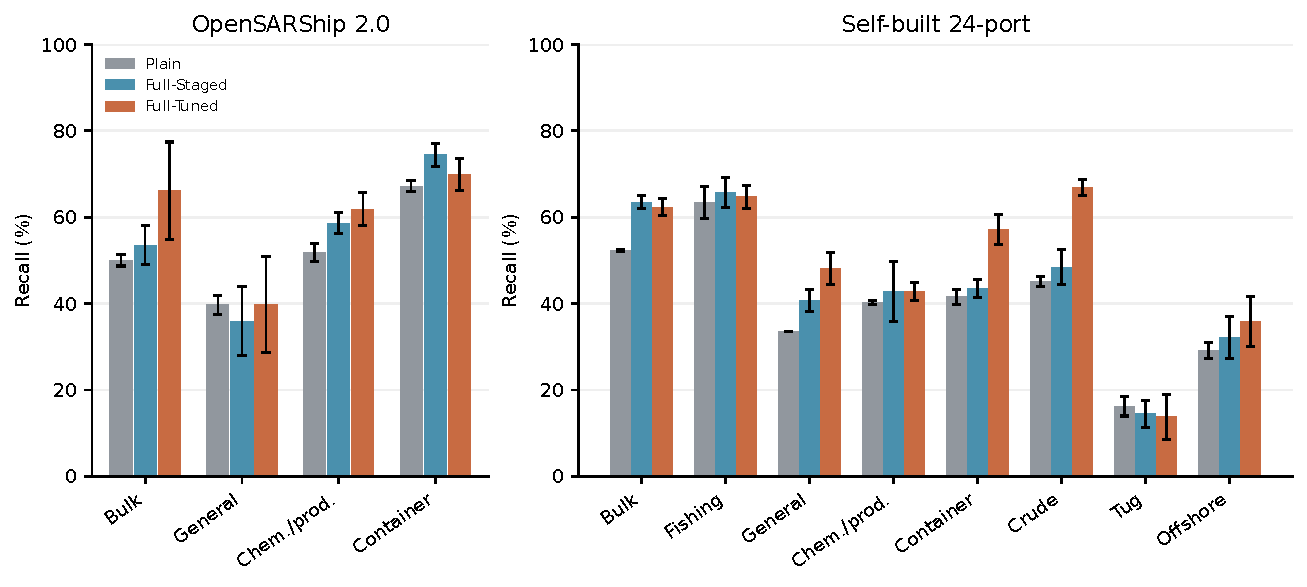
\includegraphics[width=\linewidth,height=.40\textheight,keepaspectratio]{figures/results_20261112/per_class_recall.pdf}
\caption{两个数据集的逐类召回率。Plain为分阶段普通骨干，Full-Staged为分阶段完整模型，Full-Tuned为全骨干微调完整模型；柱高与误差棒分别为种子17、29、43的均值与样本标准差。三者使用相同测试观测和原始极化可用性，训练协议见第5.2节。}
\label{fig:6}
\end{figure*}

\subsection{分阶段训练的组件消融}\label{ux5206ux9636ux6bb5ux8badux7ec3ux7684ux7ec4ux4ef6ux6d88ux878d}

表8在OSS2中分别移除一个组件，保留其余结构、共同起点和训练阶段，并重新训练。删除RGRP同时取消相应区域读出及引导接口，删除CRFB或RCEW则移除对应反馈或参考路径。

\begin{table}[H]
\centering\footnotesize
\setcounter{table}{7}
\caption{分阶段训练协议下的组件删除重训，三种子均值与标准差。}
\label{tab:8}
\setlength{\tabcolsep}{3pt}\renewcommand{\arraystretch}{1.2}
\begin{tabularx}{\linewidth}{LCCC}
\toprule
数据集 & 配置 & OA（\%） & BA（\%） \\
\midrule
OSS2 & 无CRFB & 60.670 ± 1.305 & \textbf{56.554 ± 1.239} \\
OSS2 & 无RGRP & 56.261 ± 0.666 & 52.164 ± 0.744 \\
OSS2 & 无RCEW & \textbf{61.023 ± 0.929} & 56.477 ± 0.991 \\
OSS2 & 完整模型 & \textbf{61.023 ± 2.610} & 55.630 ± 3.498 \\
自建24港 & 完整模型 & 48.412 ± 1.203 & 43.902 ± 0.654 \\
\bottomrule
\end{tabularx}
\end{table}

RGRP的贡献最明确：完整模型相对无RGRP的OA/BA提高4.762/3.466个百分点，三个种子均为正，OA船级95\%区间为{[}1.046,8.444{]}个百分点。化学品／成品油轮和集装箱船召回分别提高6.827和6.569个百分点，表明区域取证有效补充了这两类的判别信息。

CRFB和RCEW的完整重训增量较小，二者的作用进一步通过对应关系替换及消息形式比较分析。对同一完整模型开启RCEW，OSS2平均OA变化为+1.235个百分点、BA为−0.136个百分点，合计40次纠错和26次误伤。路径贡献与删除后重训的差别表明，需要结合具体证据利用过程解释组件效用。

\subsection{响应引导区域池化}\label{ux54cdux5e94ux5f15ux5bfcux533aux57dfux6c60ux5316}

保持上游、参考库和样本流一致，比较区域均值补充、从局部内容新学习注意的补充、以及复用CRFB类别响应的补充。均值对照重复四份均值摘要以匹配接口，内容注意另有4096个评分参数；其有效表达能力和初始化来源仍有差别，比较首先检验已有类别响应是否值得复用。

\begin{table}[H]
\centering\footnotesize
\setcounter{table}{8}
\caption{OSS2测试集上的区域读出比较，固定上游、三次末阶段训练。}
\label{tab:9}
\setlength{\tabcolsep}{3pt}\renewcommand{\arraystretch}{1.2}
\begin{tabularx}{\linewidth}{LCCC}
\toprule
读出方式 & OA（\%） & BA（\%） & NLL \\
\midrule
增加补充读出前的固定上游 & 62.434 & 59.718 & 1.14782 \\
区域均值补充 & 61.464 ± 0.305 & 58.233 ± 0.710 & 1.14277 \\
普通内容注意补充 & 61.464 ± 0.666 & 58.050 ± 0.674 & 1.14460 \\
CRFB响应引导RGRP补充 & \textbf{62.346 ± 0.153} & \textbf{59.781 ± 0.220} & \textbf{1.14005} \\
\bottomrule
\end{tabularx}
\end{table}

响应引导相对均值补充的OA/BA分别提高0.882/1.548个百分点，三个种子均为正；相对内容注意提高0.882/1.731个百分点。相对固定上游则为−0.088/+0.063个百分点，表明类别响应在新增区域读出中更有效地保留了原有判别能力。验证集三个方案的平均OA/BA均为62.281\%/55.731\%。

\subsection{正确空间对应是否参与判断}\label{ux6b63ux786eux7a7aux95f4ux5bf9ux5e94ux662fux5426ux53c2ux4e0eux5224ux65ad}

在响应引导模型权重固定时，将区域内部权重改成均匀值，或反向置换非空位置的权重。均匀替换保持归一化总量但改变权重分布；位置置换同时保持总量与直方图，仅改变权重与局部特征的对应。

\begin{table}[H]
\centering\footnotesize
\setcounter{table}{9}
\caption{同权重取证方式替换，OSS2测试集378条。}
\label{tab:10}
\setlength{\tabcolsep}{3pt}\renewcommand{\arraystretch}{1.2}
\begin{tabularx}{\linewidth}{LLL}
\toprule
取证方式 & OA（\%） & BA（\%） \\
\midrule
正确响应位置 & 62.346 & 59.781 \\
区域内均匀权重 & 61.464 & 57.753 \\
区域内位置置换 & 60.758 & 57.297 \\
关闭新增读出 & 62.169 & 58.796 \\
\bottomrule
\end{tabularx}
\end{table}

正确响应相对位置置换平均提高OA 1.587、BA 2.484个百分点，表明该测试队列中的正确权重---特征对应实际参与分类。响应引导相对配套均值模型共有10次纠错、0次误伤，涉及7条观测、7艘船和3个过境；其中9次在增加读出前已正确，所以主要作用是减少不合适读出适配造成的损失。

图7中普通货船000133的真实类分差，在均值读出下为−0.06155，响应引导下为+0.22820；同权重均匀替换和位置置换后分别为−0.06187与−0.13565。该样本关闭新增读出时仍正确，说明优势来自更合适的区域取证。线性分解中，VV框内、轴端与侧向对普通货船相对油轮的优势贡献分别约+0.0860、+0.0449和+0.1778，VH三项为负，体现了极化及区域作用的差异。

\begin{figure}[!htb]
\centering
\setcounter{figure}{6}
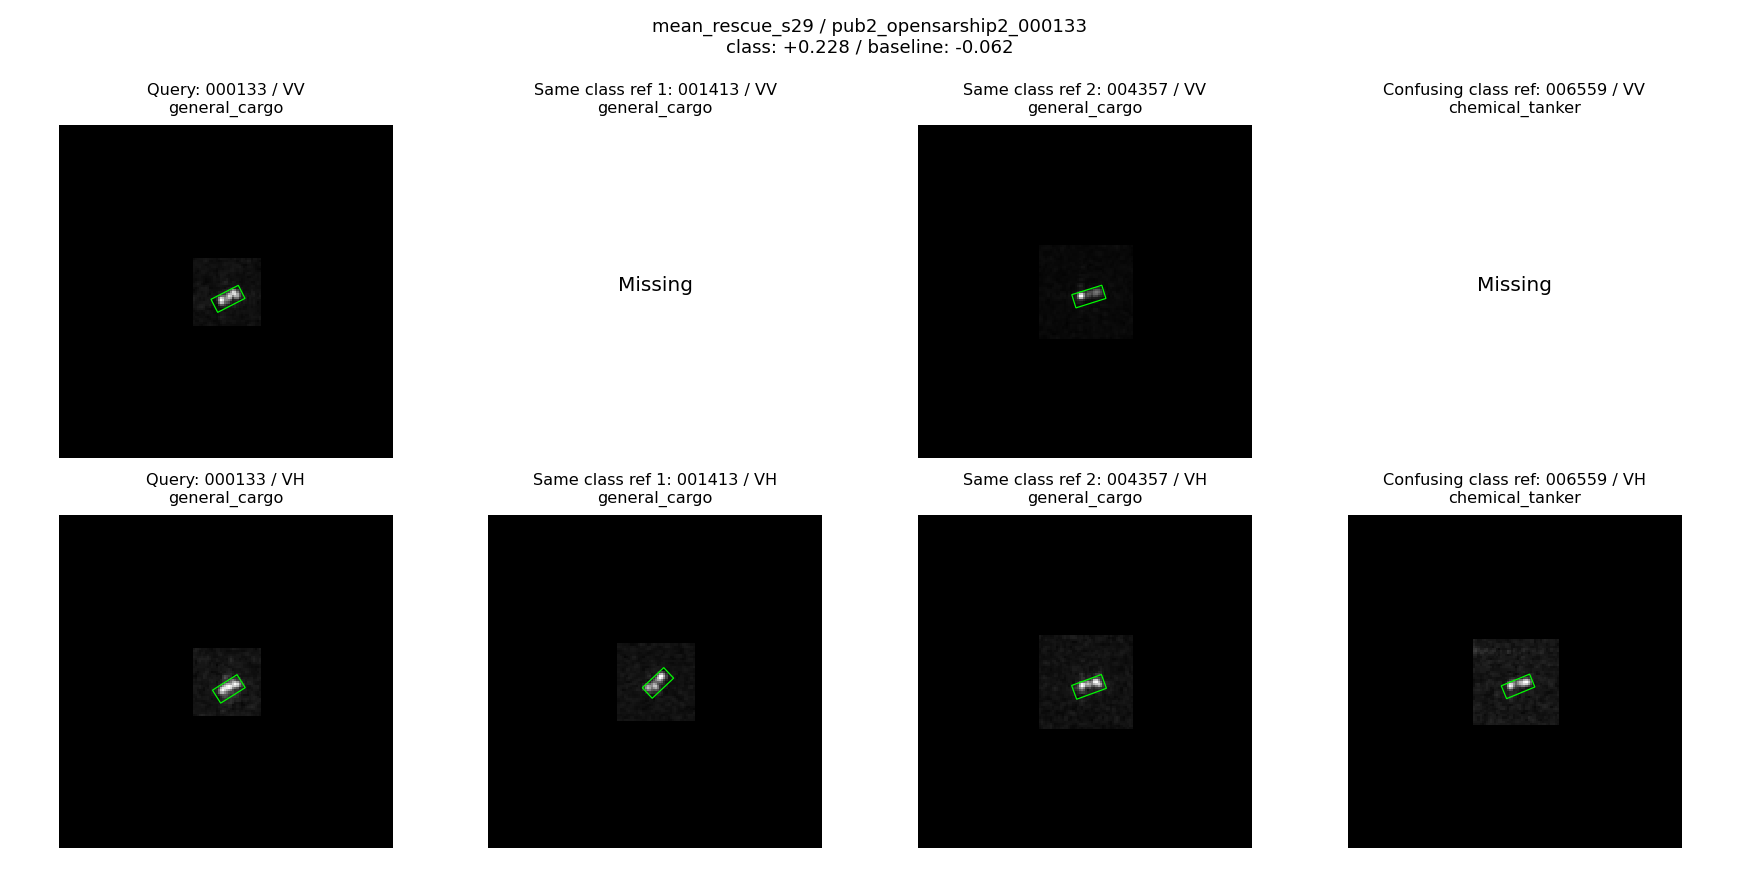
\includegraphics[width=\linewidth,height=.30\textheight,keepaspectratio]{figures/fig6_m1_m2_case.png}
\caption{普通货船000133及合法参考的VV/VH图像。baseline为均值读出对照；Missing表示该极化未通过输入有效性筛选。图像按原生尺度裁剪或补零。}
\label{fig:7}
\end{figure}

\subsection{参考证据的消息形式}\label{ux53c2ux8003ux8bc1ux636eux7684ux6d88ux606fux5f62ux5f0f}

在固定前端的独立RCEW实验中，三组配对训练使用相同源数据、查询／参考episode和120步预算，仅更新相应参考模块及分类头。表11采用相同训练长度下的末轮结果。

\begin{table}[H]
\centering\footnotesize
\setcounter{table}{10}
\caption{RCEW独立训练的验证集比较，固定前端、三种子平均。}
\label{tab:11}
\setlength{\tabcolsep}{3pt}\renewcommand{\arraystretch}{1.2}
\begin{tabularx}{\linewidth}{LLL}
\toprule
方案 & OA（\%） & BA（\%） \\
\midrule
无RCEW，更新分类头 & 58.626 ± 0.253 & 50.017 ± 0.162 \\
普通参考特征回写 & 58.772 ± 0.439 & 50.119 ± 0.281 \\
类别证据回写，精细对应 & 60.234 ± 1.410 & 51.830 ± 0.852 \\
类别证据回写，保留边际聚合 & \textbf{61.257 ± 2.251} & \textbf{53.511 ± 2.442} \\
\bottomrule
\end{tabularx}
\end{table}

聚合证据回写相对无RCEW提高OA/BA 2.632/3.495个百分点，相对普通参考特征回写提高2.485/3.392个百分点。普通参考特征回写仍保留类别、区域和极化组织，因此这一比较不只是``有类别信息''对``完全无组织信息''。图8的集装箱船000867在三个种子中均被类别证据回写判对，而普通参考回写、无RCEW和其自身关闭回写均错。seed17的真实类分差由无RCEW的−0.334、参考特征回写的−0.286变为+0.275，构成直接路径案例。

\begin{figure}[!htb]
\centering
\setcounter{figure}{7}
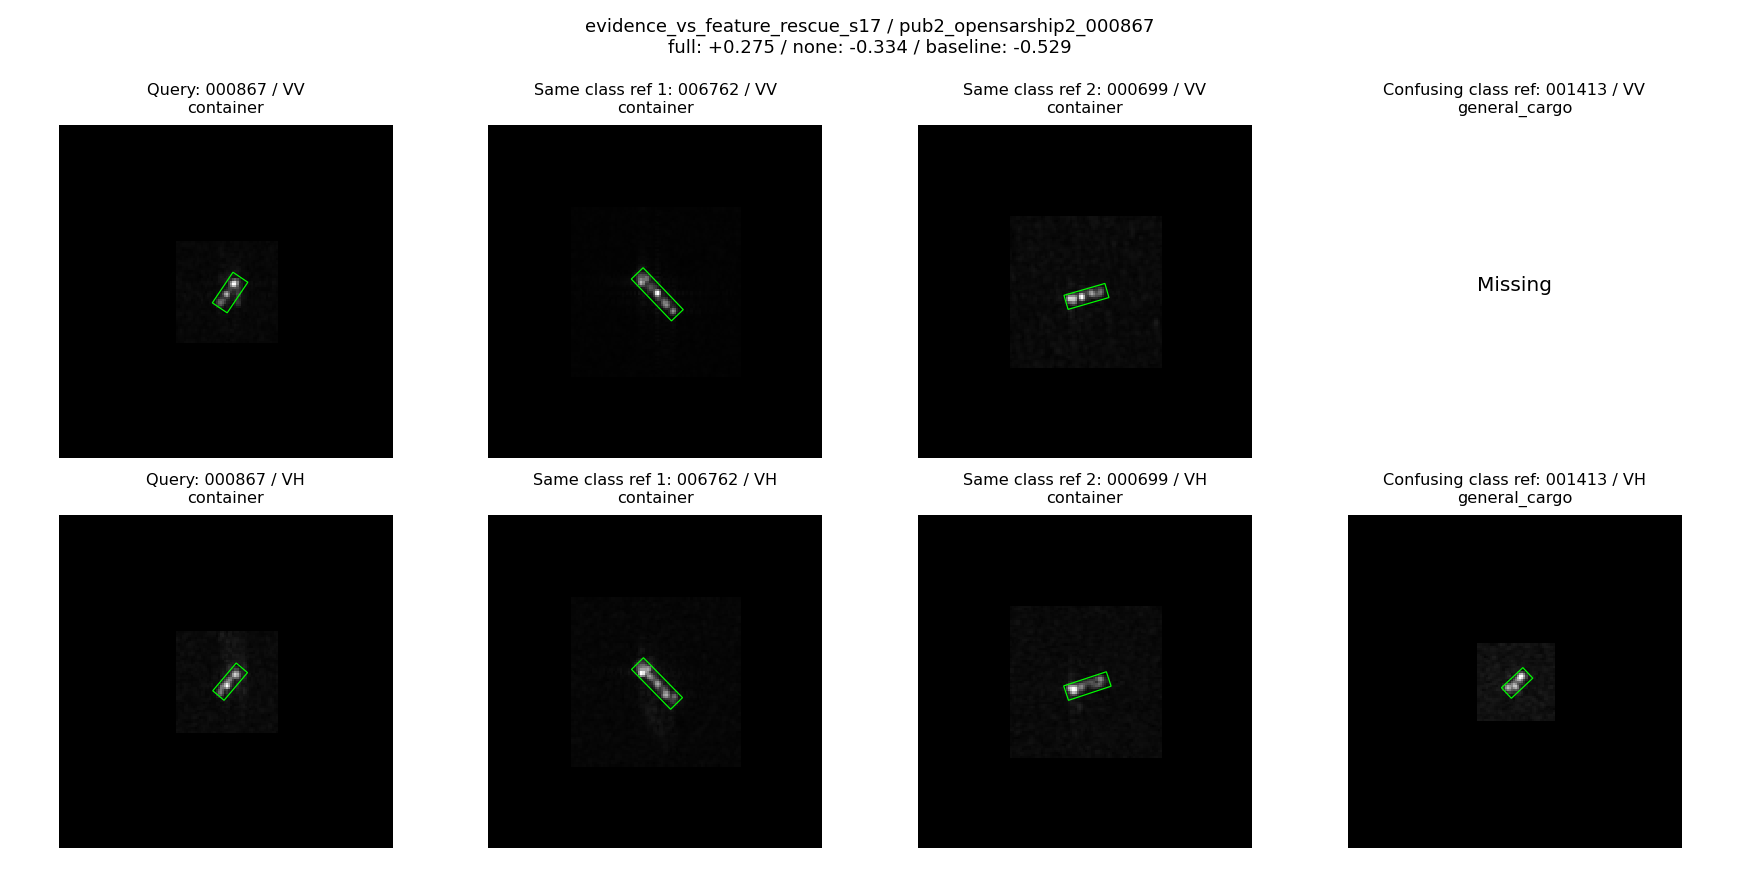
\includegraphics[width=\linewidth,height=.30\textheight,keepaspectratio]{figures/fig7_m3_case.png}
\caption{集装箱船000867及同类、混淆类参考。full为类别证据回写，none为关闭参考模块，baseline为图示原始基线。样本在三次训练中均由类别证据回写判对。}
\label{fig:8}
\end{figure}

图9进一步呈现参考信息进入查询特征的空间路径。在早期空间回写配置的八分类、16源参考诊断中，Jebel Ali散货船12457的真实类分差由关闭回写时的−0.836变为+0.138；移除VH整路回写后降至−0.486，单独移除VH框内回写后为−0.250。该路径干预将分类变化定位到实际回写响应，而非仅凭匹配热图解释。

\begin{figure}[!htb]
\centering
\setcounter{figure}{8}
\includegraphics[width=\linewidth,height=.30\textheight,keepaspectratio]{figures/author_20261110/fig12_author.pdf}
\caption{空间参考回写的路径诊断。上方为散货船12457、同类参考31512与混淆类参考13000的VH图像及区域位置，下方为局部软对应、16个参考的聚合权重和查询回写强度。该图取自早期空间回写配置，展示参考比较至特征更新的过程；当前类别证据回写的效果见图8。}
\label{fig:9}
\end{figure}

对精细对应模型保持权重并改用边际聚合，三个种子、228条查询的预测均不变；配套训练的聚合版平均表现更好。保留类别关系与参考选择后，区域聚合已能提供有效的回写消息。

在全骨干微调模型上，进一步固定权重、原图和32个源参考，对实际聚合回写路径进行干预。原路径的OA／BA为64.727\%／59.396\%，同权重关闭回写为64.374\%／59.702\%，使用简单类别均值替代为64.109\%／58.664\%。原路径相对简单均值平均提高OA 0.617、BA 0.732个百分点；相对无回写则出现OA小幅提高、BA小幅降低，反映收益在类别间的不同分配。该比较定位已训练路径的作用，不等同于删除模块后重新训练。

对应案例中，查询002422（seed29）的真实类分差为+0.0928，改用简单类别均值后为−0.0769，撤除框内回写后为−0.0545，说明该样本需要当前框内证据组织才能越过判别边界。对图9的历史样本12457，撤除VV或VH轴端回写分别将分差从+0.13756降至+0.10698或+0.10911，仍保持正确。这一区别表明局部回写既可能决定预测翻转，也可能只增加已有判断的余量；更新热图的幅度与其分类贡献需结合路径撤除共同解释。

\subsection{固定上游下的参考与读出协同}\label{ux56faux5b9aux4e0aux6e38ux4e0bux7684ux53c2ux8003ux4e0eux8bfbux51faux534fux540c}

固定相同上游，移除RCEW残差后重新计算layer4与深层区域摘要，再以相同初始化、源样本顺序和180步预算训练区域补充及分类头。保留RCEW的组合沿用表9结果。此对照比较固定上游条件下、有无参考证据时的配套末阶段优化，不等同于表8的共同起点完整重训。

\begin{table*}[!t]
\centering\footnotesize
\setcounter{table}{11}
\caption{固定上游下有无RCEW的末阶段配套训练比较。}
\label{tab:12}
\setlength{\tabcolsep}{3pt}\renewcommand{\arraystretch}{1.2}
\begin{tabularx}{\linewidth}{LCCCC}
\toprule
队列 & 配置 & OA（\%） & BA（\%） & NLL \\
\midrule
验证集228 & 无RCEW配套训练 & 61.404 ± 0.439 & 54.581 ± 0.287 & 1.23567 \\
验证集228 & 保留RCEW & 62.281 ± 0.439 & 55.731 ± 0.284 & 1.23337 \\
测试集378 & 无RCEW配套训练 & 61.993 ± 0.808 & 59.020 ± 0.951 & 1.14967 \\
测试集378 & 保留RCEW & 62.346 ± 0.153 & 59.781 ± 0.220 & 1.14005 \\
\bottomrule
\end{tabularx}
\end{table*}

RCEW在验证集与测试集上的平均OA/BA增量分别为+0.877/+1.149和+0.353/+0.760个百分点。测试集三个种子的NLL均下降，平均降低0.00963，说明在该固定上游和配套读出设置下，参考证据能提供小幅净收益。

测试集三次训练合计13次纠错与9次误伤，涉及8艘与6艘船。集装箱船002950在seed17下的真实类分差由无RCEW配套模型的−0.07493提高至+0.36983，同权重关闭回写亦会误判。这一案例将参考证据的作用落实为正确类相对竞争类的优势恢复。

\subsection{计算成本与推理加速}\label{ux8ba1ux7b97ux6210ux672cux4e0eux63a8ux7406ux52a0ux901f}

计算成本在RTX 5050 Laptop GPU（8 GB）上测量，采用FP32、关闭TF32，输入为双极化 \(160\times160\) chip。计时覆盖GPU上的图像及掩膜到分类分数的完整前向，不含检测、文件读取和CPU预处理。下述受限骨干版本的加速实现缓存32个源参考描述子，并将RCEW固定形状的60步传输迭代捕获为CUDA Graph。该计时对应固定检查点及专用图重放路径，不作为最终全骨干微调模型运行路径的实测延迟。延迟均在预热后测量并取中位数：普通骨干和SE各三组、每组15次，完整模型各三组、每组10次。

\begin{table}[H]
\centering\footnotesize
\setcounter{table}{12}
\caption{分阶段四分类模型的在线计算成本。运算量仅统计卷积与矩阵乘，一次乘加计两次操作。}
\label{tab:13}
\setlength{\tabcolsep}{3pt}\renewcommand{\arraystretch}{1.2}
\begin{tabularx}{\linewidth}{LCCCC}
\toprule
方法 & 参数（M） & 运算量（G） & 延迟（ms） & 显存（MiB） \\
\midrule
普通骨干 & 23.524 & 8.342 & 6.51 & 158.7 \\
匹配位置SE & 23.690 & 8.343 & 7.50 & 161.5 \\
本文完整模型 & 25.053 & 8.673 & 49.37 & --- \\
\bottomrule
\end{tabularx}
\end{table}

参数量统计实际执行的网络参数，显存为PyTorch在线分配峰值。完整模型增加6.50\%的执行参数和3.96\%的卷积／矩阵乘运算量；后者未覆盖归一化及传输迭代等操作。参考缓存占3.755 MiB，一次构建耗时43.43 ms。

完整模型的单张稳态延迟为49.37 ms；批量8的整批延迟为63.87 ms，吞吐达125.3张/s。图重放不改变模型权重和数值精度，OSS2同一种子的378条预测类别全部保持一致。稳态计时不含参考库构建和一次性图初始化；单张配置的图初始化约0.683 s。

\subsection{核心算子的配套替换}\label{ux6838ux5fc3ux7b97ux5b50ux7684ux914dux5957ux66ffux6362}

表14进一步分解CRFB的均值反馈与类别关系反馈，以及RCEW的通道度量与类别竞争偏置。CRFB对照保留类别响应读出、辅助监督及RGRP引导接口，仅关闭指定反馈支路；因此无反馈配置不同于表8的整块删除。RCEW的单位度量对照将通道权重固定为1，无竞争偏置对照将相应项置零，其余参考比较和回写路径保持不变。各配置从对应机制启用前的共同检查点开始，重新训练受影响阶段及后续阶段；训练步数、源参考成员和样本顺序保持一致，干预与源难例权重沿用相同生成规则。已有表9---12的固定上游结果与本表分开比较。

\begin{table}[H]
\centering\footnotesize
\setcounter{table}{13}
\caption{核心算子替换的测试集结果。各数据集单元格为三种子平均OA／BA（\%）。}
\label{tab:14}
\setlength{\tabcolsep}{3pt}\renewcommand{\arraystretch}{1.2}
\begin{tabularx}{\linewidth}{LCCC}
\toprule
组件 & 替换方式 & OSS2 & 自建24港 \\
\midrule
CRFB & 无反馈，保留响应读出 & 60.670／55.897 & --- \\
CRFB & 仅均值反馈 & 60.935／55.606 & --- \\
CRFB & 仅类别关系反馈 & 60.317／55.619 & --- \\
CRFB & 均值＋类别关系反馈 & 61.023／55.630 & --- \\
RGRP & 同范围内外合并池化 & 60.847／57.221 & --- \\
RGRP & 保留内部区域，仅合并最终读出 & 61.640／58.086 & --- \\
RGRP & 分区域池化，内部回写＋末端读出 & 61.023／55.630 & 48.412／43.902 \\
RCEW & 参考类别证据回写 & 61.023／55.630 & 48.412／43.902 \\
RCEW & 单位通道度量，无竞争偏置 & 60.847／56.060 & --- \\
RCEW & 学习通道度量，无竞争偏置 & 61.199／56.311 & --- \\
RCEW & 单位通道度量，保留竞争偏置 & 60.847／56.716 & --- \\
RCEW & 学习通道度量＋竞争偏置 & 61.023／55.630 & --- \\
\bottomrule
\end{tabularx}
\end{table}

CRFB双反馈相对仅均值反馈的平均OA和BA分别提高0.088和0.024个百分点，相对仅类别关系反馈的OA提高0.705个百分点、BA基本持平。均值与关系分支的组合能够保留部分边界样本的判别优势，但本设置下额外平均收益较小。该结果与表9的响应引导收益对应不同作用位置：前者衡量中间特征反馈，后者衡量类别响应在区域取证中的复用。

RGRP的区域身份比较保持图像覆盖范围和局部处理路径不变。保留内部区域回写、仅合并最终读出，相对内外全部合并提高OA 0.794、BA 0.865个百分点，三个种子的BA均提高；相比之下，最终三区域读出并未在测试集上优于合并读出。因此，RGRP相对整块删除的收益来自局部取证与回写的组合，内部区域组织具有增量，而不宜把全部收益归因于最终描述中的三区域区分。原区域配置在验证集上的BA为57.582\%，高于仅合并最终读出的53.572\%，模型选择仍沿用验证集结果。

RCEW在关闭竞争偏置时，学习通道度量相对单位度量提高OA 0.353、BA 0.250个百分点，三个种子的BA增量均为正。加入竞争偏置后，平均OA和BA分别较仅通道度量下降0.176和0.681个百分点，说明两个机制的收益并非简单相加。因而，类别比较与参考回写的有效性应结合表11---12的消息形式和路径对照解释，而不能仅以内部组件数量说明优势。

\subsection{极化处理方式}\label{ux6781ux5316ux5904ux7406ux65b9ux5f0f}

极化参数比较保持共享ResNet-50骨干、模块位置、训练阶段及输入可用性不变，仅改变极化对应模块的参数绑定方式。每个种子先把VV初始化复制给VH，使共享组与专属组从相同初始函数出发；两组均完成736次更新并使用配对的样本顺序。参数共享作用于CRFB、RGRP的可训练变换及RCEW的极化对应变换，原本共用的度量部分保持不变。两组使用相同378条测试观测，而非分别挑选可用样本。

\begin{table}[H]
\centering\footnotesize
\setcounter{table}{14}
\caption{极化输入与参数组织比较。各数据集单元格为OA／BA（\%）。}
\label{tab:15}
\setlength{\tabcolsep}{3pt}\renewcommand{\arraystretch}{1.2}
\begin{tabularx}{\linewidth}{LCCC}
\toprule
输入 & 参数组织 & OSS2 & 自建24港 \\
\midrule
VV＋VH & 共享骨干、共享模块 & 59.965／53.971 & --- \\
VV＋VH & 共享骨干、极化专属模块 & \textbf{61.376／56.252} & --- \\
\bottomrule
\end{tabularx}
\end{table}

极化专属参数相对共享参数提高OA 1.411、BA 2.281个百分点，三个种子的BA均提高；在两路均可用的348条子集中，仍提高OA 0.766、BA 1.514个百分点。普通货船召回提高6.410个百分点，是主要BA收益来源。该结果支持共享通用骨干、允许极化相关证据变换分别学习的组织方式；它评价的是整体参数策略，包含新增参数容量的作用，而非证明每个模块都必须独立处理两种极化。

针对一侧未获得有效OBB的输入，另固定微调完整模型与原参考，在核实两极化裁片的地理对应及裁剪映射后，用可用极化的目标框恢复另一视图。OSS2的30条单路测试观测均具有对应原图，仅恢复查询后全测试OA由64.727\%提高至65.344\%，BA由59.396\%变为59.430\%；同时恢复查询和参考后为65.785\%和59.776\%。在自建24港，恢复83条测试观测的缺失视图后，OA与BA由52.076\%／48.970\%提高至52.249\%／49.481\%；进一步恢复参考视图后为52.379\%／49.691\%。两数据集均固定各自微调权重，输入恢复结果独立于表7报告。定位可用性能够影响识别，但不是所有误分类的共同原因。

\subsection{干预指导训练}\label{ux5e72ux9884ux6307ux5bfcux8badux7ec3}

表16在完整训练的干预适配阶段替换选样方式，再执行相同的参考、类别反馈和区域读出训练。普通适配仅使用原图分类监督与教师正确样本的分布保持；随机选样与干预选样使用相同判别优势保护，并按类别匹配选样数量。比较保持更新参数、训练预算和后续阶段一致，检验选样机制对最终分类的作用。

\begin{table}[H]
\centering\footnotesize
\setcounter{table}{15}
\caption{完整训练路径内的干预指导对照。各数据集单元格为三种子平均OA／BA（\%）。}
\label{tab:16}
\setlength{\tabcolsep}{3pt}\renewcommand{\arraystretch}{1.2}
\begin{tabularx}{\linewidth}{LCCC}
\toprule
适配方式 & 判别优势保护对象 & OSS2 & 自建24港 \\
\midrule
普通适配 & 无 & 60.141／54.866 & --- \\
类内配额随机选样 & 随机选中的源样本 & 60.141／55.297 & --- \\
干预有效性选样 & 通过干预筛选的源样本 & \textbf{61.023／55.630} & --- \\
\bottomrule
\end{tabularx}
\end{table}

干预选样相对类内配额随机选样提高OA 0.882、BA 0.333个百分点，三个种子的OA均提高；相对无分差保护提高OA 0.882、BA 0.764个百分点。前一比较在五个测试过境中有四个取得平均OA增量，说明收益不只出现在单个场景。其船级配对OA增量95\%区间为{[}−0.440,2.216{]}个百分点，故这一结果支持小幅净收益，不作显著提升判断。

三种策略均训练全部源图像，只改变额外分差保护的分配。干预筛选的保护项在各96步适配中有89、88、90步非零，确认约束实际参与优化。化学品／成品油轮000141在两个种子中被干预选样模型救回；seed17下，相对随机选样的真实类分差由−0.678提高至+0.176。该例说明样本保护能通过后续完整训练转化为判别改善，而非要求预测时修改输入图像。

\subsection{分场景表现与定位鲁棒性}\label{ux5206ux573aux666fux8868ux73b0ux4e0eux5b9aux4f4dux9c81ux68d2ux6027}

表17按过境和港口汇总分阶段完整模型相对普通骨干的配对增量，保留不同场景的类别覆盖；场景BA仅在该组实际存在的类别上计算。表中平均增量先在每个场景内对三个训练种子取均值，再对场景等权汇总，不同于表7按全部测试观测统计的OA。自建数据的过境统计采用包含datatake的85个完整过境组。定位鲁棒性另固定图像和标签，仅改变OBB并重新生成局部区域，避免把输入像素变化与区域组织误差混为一谈。

\begin{table*}[!t]
\centering\footnotesize
\setcounter{table}{16}
\caption{场景级增量分布。增量相对普通骨干，以百分点计；正／平／负为场景数。}
\label{tab:17}
\setlength{\tabcolsep}{3pt}\renewcommand{\arraystretch}{1.2}
\begin{tabularx}{\linewidth}{LCCCC}
\toprule
数据集／分组 & 场景数 & 平均 \(\Delta\)OA & 平均 \(\Delta\)BA & OA正／平／负 \\
\midrule
OSS2／过境 & 5 & +5.199 & +7.322 & 4／0／1 \\
自建24港／过境 & 85 & +3.813 & +2.183 & 58／3／24 \\
自建24港／港口 & 18 & +1.876 & +0.088 & 12／0／6 \\
\bottomrule
\end{tabularx}
\end{table*}

完整模型在自建数据的12个港口和58个完整过境组中取得平均OA增益，其中10个港口、35个过境组在三个种子中均提高。Port Klang、Santos与Richards Bay相对普通骨干的OA分别提高6.52、10.04和9.91个百分点，说明收益分布于多个水域。场景内的类别构成仍会影响增量：Singapore的OA提高6.49个百分点，而BA下降3.72个百分点；Jebel Ali的OA下降0.16个百分点，BA提高1.24个百分点。因此，跨场景净收益与各场景内部的类别收益分配需要分别评价。这里的逐港统计对应受限骨干版本，基于同一跨场景划分，不等同于留一港训练。

\begin{table}[H]
\centering\footnotesize
\setcounter{table}{17}
\caption{固定分阶段模型的RGRP定位扰动结果。OSS2使用相同378条查询，单元格为三种子平均OA／BA（\%）。}
\label{tab:18}
\setlength{\tabcolsep}{3pt}\renewcommand{\arraystretch}{1.2}
\begin{tabularx}{\linewidth}{>{\hsize=.8\hsize}L>{\hsize=1.0\hsize}C>{\hsize=1.4\hsize}C>{\hsize=.8\hsize}C}
\toprule
比较类型 & 输入条件 & OSS2 & 自建24港 \\
\midrule
基准 & 原始OBB & 61.023／55.630 & --- \\
中心位置 & 沿轴−20\%／+20\% & \shortstack{62.346／57.338\\60.317／55.678} & --- \\
中心位置 & 横轴−20\%／+20\% & \shortstack{61.728／55.681\\60.406／54.870} & --- \\
长宽尺度 & 等比−20\%／+20\% & \shortstack{58.995／56.057\\62.610／56.221} & --- \\
长度 & −20\%／+20\% & \shortstack{59.524／56.324\\62.434／56.061} & --- \\
宽度 & −20\%／+20\% & \shortstack{60.141／55.369\\60.317／55.245} & --- \\
轴向角度 & −20°／+20° & \shortstack{61.464／56.936\\61.993／55.768} & --- \\
\bottomrule
\end{tabularx}
\end{table}

中心位移分别按框长和框宽归一化，并比较5\%、10\%、20\%的正负偏移；尺寸改变包括10\%、20\%的独立长宽及等比变化，角度比较正负5°、10°、20°，合计30个非零条件与零扰动。表18列出各变量的最大幅度，较小扰动保留相同定义。所有条件只更新查询的RGRP局部区域，图像像素、参考描述及RCEW回写保持固定，因此衡量的是区域定位敏感性，而不是整个检测流程的误差传播。

30个非零条件的平均OA变化为−2.028至+1.587个百分点，BA变化为−0.760至+1.708个百分点。缩框和扩框产生不同类别权衡：等比缩小20\%使集装箱船平均召回降低7.056个百分点、化学品／成品油轮提高8.434个百分点。故小幅总体变化并不代表每个预测不变，扩大范围也不是统一最优策略。该实验保留原框作为评价基准，不根据测试扰动择优修改输入。

\subsection{优化范围与训练成本}\label{ux4f18ux5316ux8303ux56f4ux4e0eux8badux7ec3ux6210ux672c}

表19列出分阶段完整模型与两种全骨干配置的优化结果，验证集用于选择范围、学习率与检查点，测试性能见表7。完整模型微调不改变模块位置、参考数量和原始输入权限，改善来自新增联合优化而非增加测试信息。

\begin{table}[H]
\centering\footnotesize
\setcounter{table}{18}
\caption{两个数据集的训练方案与验证集性能。轮数按seed17／29／43排列；OA／BA为三种子平均（\%）。}
\label{tab:19}
\setlength{\tabcolsep}{3pt}\renewcommand{\arraystretch}{1.2}
\begin{tabularx}{\linewidth}{LCCC}
\toprule
配置 & 初始化 & 实际轮数 & 验证OA／BA \\
\midrule
OSS2分阶段版 & ImageNet & 五阶段固定预算 & 63.304／57.582 \\
OSS2 R50-Tuned & ImageNet & 46／49／53 & 64.035／61.110 \\
OSS2本文微调 & 对应分阶段终点 & 23／19／22 & 65.936／61.224 \\
24港本文微调 & 对应分阶段终点 & 30／27／22 & 46.250／45.037 \\
\bottomrule
\end{tabularx}
\end{table}

OSS2完整模型三个微调运行共新增1,920次更新，连同继承的三次分阶段训练合计4,128次；R50-Tuned三个运行共4,440次更新。两者的源图像暴露次数分别为96,356和106,412，均为重复训练暴露而非独立样本数。自建24港微调共新增68,019次更新，三个种子的最佳检查点分别位于第29、19和14轮；其验证BA针对实际出现的七类计算，测试BA针对八类计算。完整模型还包含参考前向、辅助监督与历史分阶段学习，更新次数不能直接换算为相同计算量。这些预算与表13的稳态推理延迟分别报告，以区分训练投入和部署开销。

\FloatBarrier
\balance
\begin{thebibliography}{99}
\bibitem{ref1}L. Huang, B. Liu, B. Li, W. Guo, W. Yu, Z. Zhang, and W. Yu. OpenSARShip: A Dataset Dedicated to Sentinel-1 Ship Interpretation. \emph{IEEE JSTARS}, 11(1):195--208, 2018. doi:10.1109/JSTARS.2017.2755672.

\bibitem{ref2}H. Xie, J. He, Z. Lu, and J. Hu. Two-Level Feature-Fusion Ship Recognition Strategy Combining HOG Features with Dual-Polarized Data in SAR Images. \emph{Remote Sensing}, 15(18):4393, 2023. doi:10.3390/rs15184393.

\bibitem{ref3}Z. Shao, T. Zhang, and X. Ke. A Dual-Polarization Information-Guided Network for SAR Ship Classification. \emph{Remote Sensing}, 15(8):2138, 2023. doi:10.3390/rs15082138.

\bibitem{ref4}J. He et al.~CPINet: Towards A Novel Cross-Polarimetric Interaction Network for Dual-Polarized SAR Ship Classification. \emph{Remote Sensing}, 16(18):3479, 2024. doi:10.3390/rs16183479.

\bibitem{ref5}N. Xie, T. Zhang, W. Guo, Z. Zhang, and W. Yu. Dual Branch Deep Network for Ship Classification of Dual-Polarized SAR Images. \emph{IEEE Trans. Geosci. Remote Sens.}, 62:1--15, 2024. doi:10.1109/TGRS.2024.3372021.

\bibitem{ref6}Z. Liu, K. Li, L. Wang, and Z. Zhang. Multi-Scale Alignment Domain Adaptation for Ship Classification in Multi-Resolution SAR Images. \emph{IEEE Trans. Autom. Sci. Eng.}, 22:4051--4062, 2025. doi:10.1109/TASE.2024.3407130.

\bibitem{ref7}L. Chen, J. Li, H. Zhong, H. Shi, Z. Yang, and W. Li. PGMNet: A Prototype-Guided Multimodal Network for Ship Recognition in SAR Images. \emph{IEEE Trans. Geosci. Remote Sens.}, 63:5215517, 2025. doi:10.1109/TGRS.2025.3583282.

\bibitem{ref8}R. C. Fong and A. Vedaldi. Interpretable Explanations of Black Boxes by Meaningful Perturbation. \emph{ICCV}, 3449--3457, 2017. doi:10.1109/ICCV.2017.371.

\bibitem{ref9}S. Hooker, D. Erhan, P.-J. Kindermans, and B. Kim. A Benchmark for Interpretability Methods in Deep Neural Networks. \emph{NeurIPS}, 32, 2019.

\bibitem{ref10}X. Hou, W. Ao, Q. Song, J. Lai, H. Wang, and F. Xu. FUSAR-Ship: Building a High-Resolution SAR-AIS Matchup Dataset of Gaofen-3 for Ship Detection and Recognition. \emph{Science China Information Sciences}, 63:140303, 2020. doi:10.1007/s11432-019-2772-5.

\bibitem{ref11}S. Zhao and H. Lang. Improving Deep Subdomain Adaptation by Dual-Branch Network Embedding Attention Module for SAR Ship Classification. \emph{IEEE JSTARS}, 15:8038--8048, 2022. doi:10.1109/JSTARS.2022.3206753.

\bibitem{ref12}Y. Shi, L. Du, Y. Guo, Y. Du, and Y. Li. Unsupervised Domain Adaptation for Ship Classification via Progressive Feature Alignment: From Optical to SAR Images. \emph{IEEE Trans. Geosci. Remote Sens.}, 62:1--17, 2024. doi:10.1109/TGRS.2024.3458937.

\bibitem{ref13}Y. Qi, L. Wang, C. Zhao, P. T. Mathiopoulos, T. Ohtsuki, and F. Adachi. SCRC-Net: A Structure-Constrained and Representation-Consistent Network for SAR Ship Classification. \emph{Pattern Recognition}, 180:114294, 2026. doi:10.1016/j.patcog.2026.114294.

\bibitem{ref14}B. Zhou, A. Khosla, A. Lapedriza, A. Oliva, and A. Torralba, ``Learning Deep Features for Discriminative Localization,'' in Proc. IEEE Conf. Comput. Vis. Pattern Recognit. (CVPR), 2016, pp.~2921-2929, doi: 10.1109/CVPR.2016.319.

\bibitem{ref15}J. Hu, L. Shen, and G. Sun, ``Squeeze-and-Excitation Networks,'' in Proc. IEEE/CVF Conf. Comput. Vis. Pattern Recognit. (CVPR), 2018, pp.~7132-7141, doi: 10.1109/CVPR.2018.00745.

\bibitem{ref16}H. Lee, H.-E. Kim, and H. Nam, ``SRM: A Style-Based Recalibration Module for Convolutional Neural Networks,'' in Proc. IEEE/CVF Int. Conf. Comput. Vis. (ICCV), 2019, pp.~1854-1862, doi: 10.1109/ICCV.2019.00194.

\bibitem{ref17}Z. Gao, J. Xie, Q. Wang, and P. Li, ``Global Second-Order Pooling Convolutional Networks,'' in Proc. IEEE/CVF Conf. Comput. Vis. Pattern Recognit. (CVPR), 2019, pp.~3024-3033, doi: 10.1109/CVPR.2019.00314.

\bibitem{ref18}Y. Chen, Y. Kalantidis, J. Li, S. Yan, and J. Feng, ``A\^{}2-Nets: Double Attention Networks,'' in Adv. Neural Inf. Process. Syst., vol.~31, 2018, pp.~352-361.

\bibitem{ref19}Y. Cao, J. Xu, S. Lin, F. Wei, and H. Hu, ``GCNet: Non-Local Networks Meet Squeeze-Excitation Networks and Beyond,'' in Proc. IEEE/CVF Int. Conf. Comput. Vis. Workshops (ICCVW), 2019, pp.~1971-1980, doi: 10.1109/ICCVW.2019.00246.

\bibitem{ref20}J. Dai, Y. Li, K. He, and J. Sun, ``R-FCN: Object Detection via Region-based Fully Convolutional Networks,'' in Adv. Neural Inf. Process. Syst., vol.~29, 2016, pp.~379-387.

\bibitem{ref21}X. Li, X. Wang, R. Zhu, Z. Ma, J. Cao, and J.-H. Xue. Selectively Augmented Attention Network for Few-Shot Image Classification. \emph{IEEE Trans. Circuits Syst. Video Technol.}, 35(2):1180--1192, 2025. doi:10.1109/TCSVT.2024.3480279.

\bibitem{ref22}J. Snell, K. Swersky, and R. Zemel, ``Prototypical Networks for Few-shot Learning,'' in Adv. Neural Inf. Process. Syst., vol.~30, 2017, pp.~4077-4087.

\bibitem{ref23}W. Li, L. Wang, J. Xu, J. Huo, Y. Gao, and J. Luo, ``Revisiting Local Descriptor Based Image-To-Class Measure for Few-Shot Learning,'' in Proc. IEEE/CVF Conf. Comput. Vis. Pattern Recognit. (CVPR), 2019, pp.~7260-7268, doi: 10.1109/CVPR.2019.00743.

\bibitem{ref24}R. Hou, H. Chang, B. Ma, S. Shan, and X. Chen, ``Cross Attention Network for Few-shot Classification,'' in Adv. Neural Inf. Process. Syst., vol.~32, 2019, pp.~4003-4014.

\bibitem{ref25}C. Zhang, Y. Cai, G. Lin, and C. Shen. DeepEMD: Few-Shot Image Classification With Differentiable Earth Mover's Distance and Structured Classifiers. \emph{CVPR}, 12203--12213, 2020.

\bibitem{ref26}D. Wertheimer, L. Tang, and B. Hariharan, ``Few-Shot Classification With Feature Map Reconstruction Networks,'' in Proc. IEEE/CVF Conf. Comput. Vis. Pattern Recognit. (CVPR), 2021, pp.~8012-8021, doi: 10.1109/CVPR46437.2021.00792.

\bibitem{ref27}J. Wu, D. Chang, A. Sain, X. Li, Z. Ma, J. Cao, J. Guo, and Y.-Z. Song. Bi-Directional Ensemble Feature Reconstruction Network for Few-Shot Fine-Grained Classification. \emph{IEEE Trans. Pattern Anal. Mach. Intell.}, 46(9):6082--6096, 2024. doi:10.1109/TPAMI.2024.3376686.

\bibitem{ref28}W. Li, W. Yang, L. Liu, W. Zhang, and Y. Liu. Discovering and Explaining the Noncausality of Deep Learning in SAR ATR. \emph{IEEE GRSL}, 20:1--5, 2023. doi:10.1109/LGRS.2023.3266493.

\bibitem{ref29}D. Yin, R. G. Lopes, J. Shlens, E. D. Cubuk, and J. Gilmer. A Fourier Perspective on Model Robustness in Computer Vision. \emph{NeurIPS}, 32, 2019.

\bibitem{ref30}A. S. Ross, M. C. Hughes, and F. Doshi-Velez. Right for the Right Reasons: Training Differentiable Models by Constraining Their Explanations. \emph{IJCAI}, 2017.

\bibitem{ref31}Z. Huang, H. Wang, E. P. Xing, and D. Huang, ``Self-challenging Improves Cross-Domain Generalization,'' in Computer Vision - ECCV 2020, Lecture Notes in Computer Science, vol.~12347, 2020, pp.~124-140, doi: 10.1007/978-3-030-58536-5\_8.

\bibitem{ref32}A. S. Ross and F. Doshi-Velez, ``Improving the Adversarial Robustness and Interpretability of Deep Neural Networks by Regularizing Their Input Gradients,'' in Proc. AAAI Conf. Artif. Intell., vol.~32, no. 1, 2018, pp.~1660-1669, doi: 10.1609/aaai.v32i1.11504.

\bibitem{ref33}P. Chattopadhyay, K. Sarangmath, V. Vijaykumar, and J. Hoffman. PASTA: Proportional Amplitude Spectrum Training Augmentation for Syn-to-Real Domain Generalization. \emph{ICCV}, 19288--19300, 2023.

\bibitem{ref34}H. Cheng, S. Yang, J. T. Zhou, L. Guo, and B. Wen. Frequency Guidance Matters in Few-Shot Learning. \emph{ICCV}, 11814--11824, 2023.

\bibitem{ref35}Y. Wang, F. Liu, Z. Chen, Y.-C. Wu, J. Hao, G. Chen, and P.-A. Heng. Contrastive-ACE: Domain Generalization Through Alignment of Causal Mechanisms. \emph{IEEE Trans. Image Process.}, 32:235--250, 2023. doi:10.1109/TIP.2022.3227457.

\bibitem{ref36}K. He, X. Zhang, S. Ren, and J. Sun. Deep Residual Learning for Image Recognition. \emph{CVPR}, 770--778, 2016.
\end{thebibliography}

\end{document}
